%
% The first command in your LaTeX source must be the \documentclass command.
\documentclass[sigconf,anonymous]{acmart}

\usepackage{bm}
\usepackage[margin=5pt]{subcaption}
\usepackage{siunitx}
%
% defining the \BibTeX command - from Oren Patashnik's original BibTeX documentation.
\def\BibTeX{{\rm B\kern-.05em{\sc i\kern-.025em b}\kern-.08emT\kern-.1667em\lower.7ex\hbox{E}\kern-.125emX}}

% このコピーライトの所は一体どうすればいいのかを確認する必要がある
% Rights management information.
% This information is sent to you when you complete the rights form.
% These commands have SAMPLE values in them; it is your responsibility as an author to replace
% the commands and values with those provided to you when you complete the rights form.
%
% These commands are for a PROCEEDINGS abstract or paper.

\copyrightyear{2018}
\acmYear{2018}
\setcopyright{acmlicensed}
\acmConference[Woodstock '18]{Woodstock '18: ACM Symposium on Neural Gaze Detection}{June 03--05, 2018}{Woodstock, NY}
\acmBooktitle{Woodstock '18: ACM Symposium on Neural Gaze Detection, June 03--05, 2018, Woodstock, NY}
\acmPrice{15.00}
\acmDOI{10.1145/1122445.1122456}
\acmISBN{978-1-4503-9999-9/18/06}

%  CEAに出す原稿はジャーナルではないはずなので無視して良さそう
% These commands are for a JOURNAL article.
%\setcopyright{acmcopyright}
%\acmJournal{TOG}
%\acmYear{2018}\acmVolume{37}\acmNumber{4}\acmArticle{111}\acmMonth{8}
%\acmDOI{10.1145/1122445.1122456}

%
% Submission ID.
% Use this when submitting an article to a sponsored event. You'll receive a unique submission ID from the organizers
% of the event, and this ID should be used as the parameter to this command.
%\acmSubmissionID{123-A56-BU3}

%
% The majority of ACM publications use numbered citations and references. If you are preparing content for an event
% sponsored by ACM SIGGRAPH, you must use the "author year" style of citations and references. Uncommenting
% the next command will enable that style.
%\citestyle{acmauthoryear}

%
% end of the preamble, start of the body of the document source.
\begin{document}


% The "title" command has an optional parameter, allowing the author to define a "short title" to be used in page headers.
\title{Cooking state recognition based on \\ Acoustic event detection}

% The "author" command and its associated commands are used to define the authors and their affiliations.
% Of note is the shared affiliation of the first two authors, and the "authornote" and "authornotemark" commands
% used to denote shared contribution to the research.
\author{Yusaku Korematsu}
\authornote{Both authors contributed equally to this research.}
\email{korematsu@gavo.t.u-tokyo.ac.jp}
\orcid{1234-5678-9012}
\author{Daisuke Satio}
\authornotemark[1]
\email{dsk-saito@gavo.t.u-tokyo.ac.jp}
\affiliation{%
  \institution{The University of Tokyo}
  \streetaddress{P.O. Box 1212}
  \city{Tokyo}
  \state{Japan}
  \postcode{43017-6221}
}

%
% By default, the full list of authors will be used in the page headers. Often, this list is too long, and will overlap
% other information printed in the page headers. This command allows the author to define a more concise list
% of authors' names for this purpose.
% \renewcommand{\shortauthors}{Trovato and Tobin, et al.}

%
% The abstract is a short summary of the work to be presented in the article.
\begin{abstract}
  % 本研究では調理支援システムに向けた,調理行動理解のための調理音解析を行なった.
  % 調理行動理解のために,画像やモーションセンサーの信号,温度センサーなどを用いる試みはあるが,音響信号を用いた研究は限定的なものしか行われていない.
  % 実際の調理を行い録音をすることで新たにデータセットを構築し実験を行なった.
  % 人間が調理を行う時,調理行動の種類によって異なる調理音が発生する.各調理音を学習しレシピ構造から行動系列を制限することで効果的に調理行動列を推定することが達成された.
  In this research, the cooking sound analysis for understanding cooking activities was conducted toward the cooking support system.
  Although there have been attempts to use images and signals from motion sensors and temperature sensors to understand cooking behavior, only limited studies have been conducted using acoustic signals.
  The data set was newly constructed by actually cooking and recording.
  When humans cook, different cooking sounds are generated depending on the type of cooking behavior. By learning each cooking sound and restricting the action sequence from the recipe structure, it was achieved to estimate the cooking action sequence effectively.
\end{abstract}

%
% The code below is generated by the tool at http://dl.acm.org/ccs.cfm.
% Please copy and paste the code instead of the example below.
%
\begin{CCSXML}
<ccs2012>
<concept>
<concept_id>10002951</concept_id>
<concept_desc>Information systems</concept_desc>
<concept_significance>300</concept_significance>
</concept>
</ccs2012>
\end{CCSXML}

\ccsdesc[300]{Information systems}

%
% Keywords. The author(s) should pick words that accurately describe the work being
% presented. Separate the keywords with commas.
\keywords{Cooking activities recognition, Acoustic event detection, Signal processing, Nonnegative matrix factorization}

%
% A "teaser" image appears between the author and affiliation information and the body
% of the document, and typically spans the page.
% \begin{teaserfigure}
%   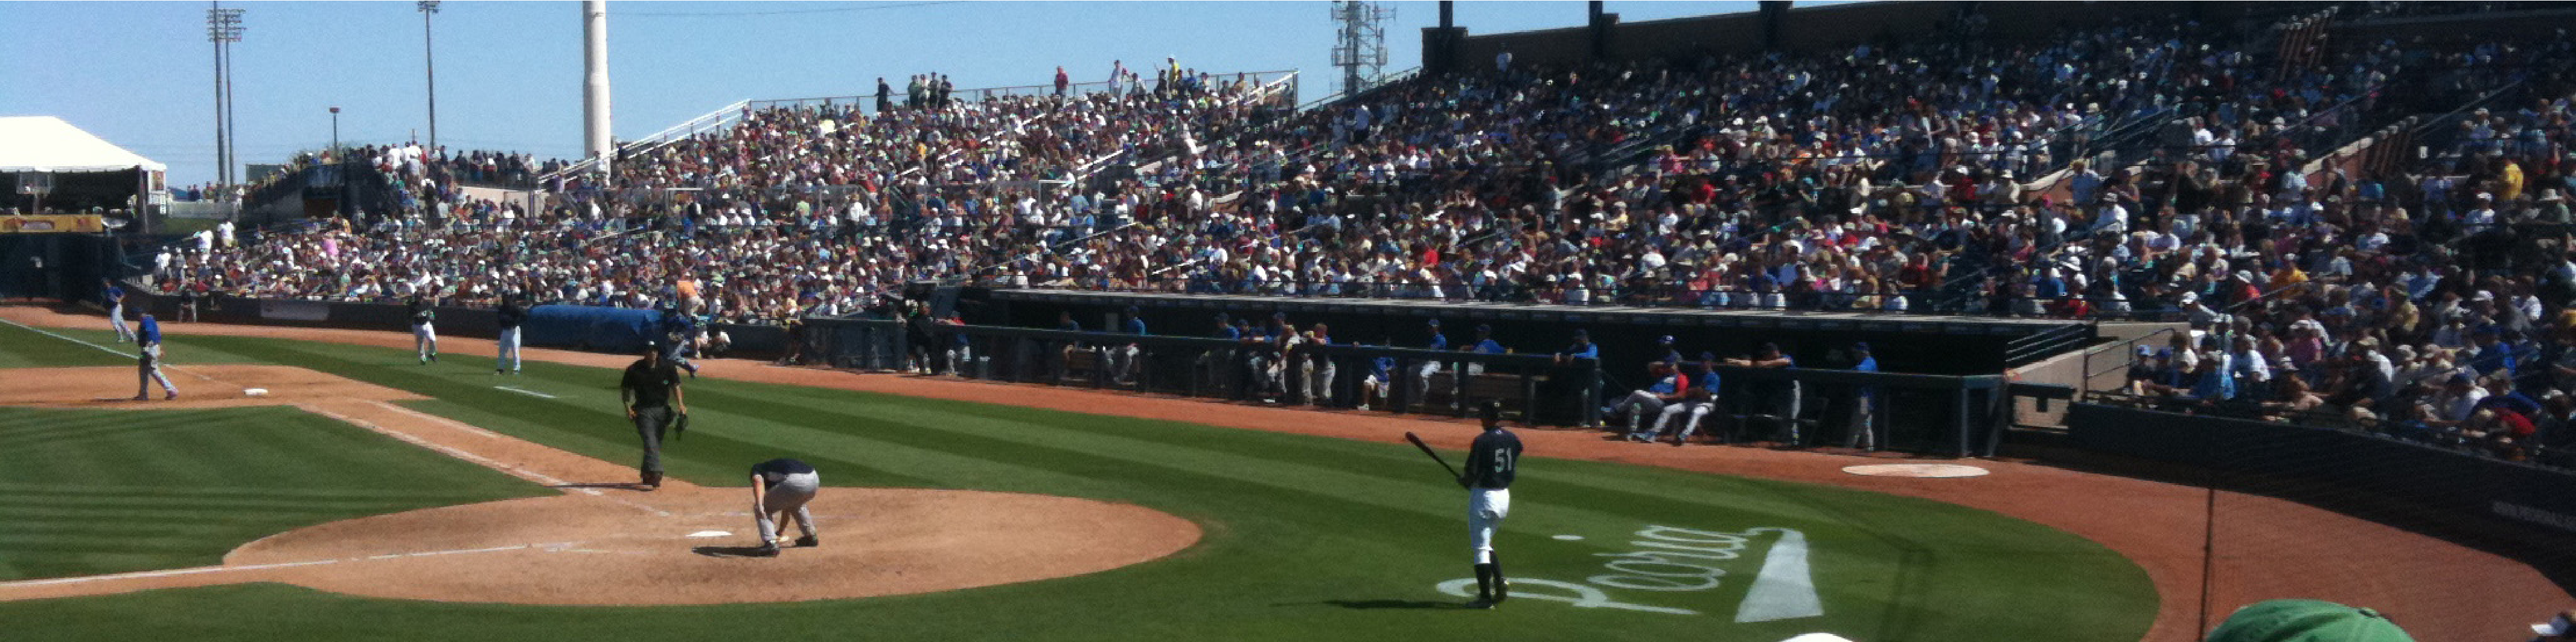
\includegraphics[width=\textwidth]{fig/sampleteaser.pdf}
%   \caption{Seattle Mariners at Spring Training, 2010.}
%   \Description{Enjoying the baseball game from the third-base seats. Ichiro Suzuki preparing to bat.}
%   \label{fig:teaser}
% \end{teaserfigure}

%
% This command processes the author and affiliation and title information and builds
% the first part of the formatted document.
\maketitle

\section{Introduction}

\begin{figure}[t]
  \centering
  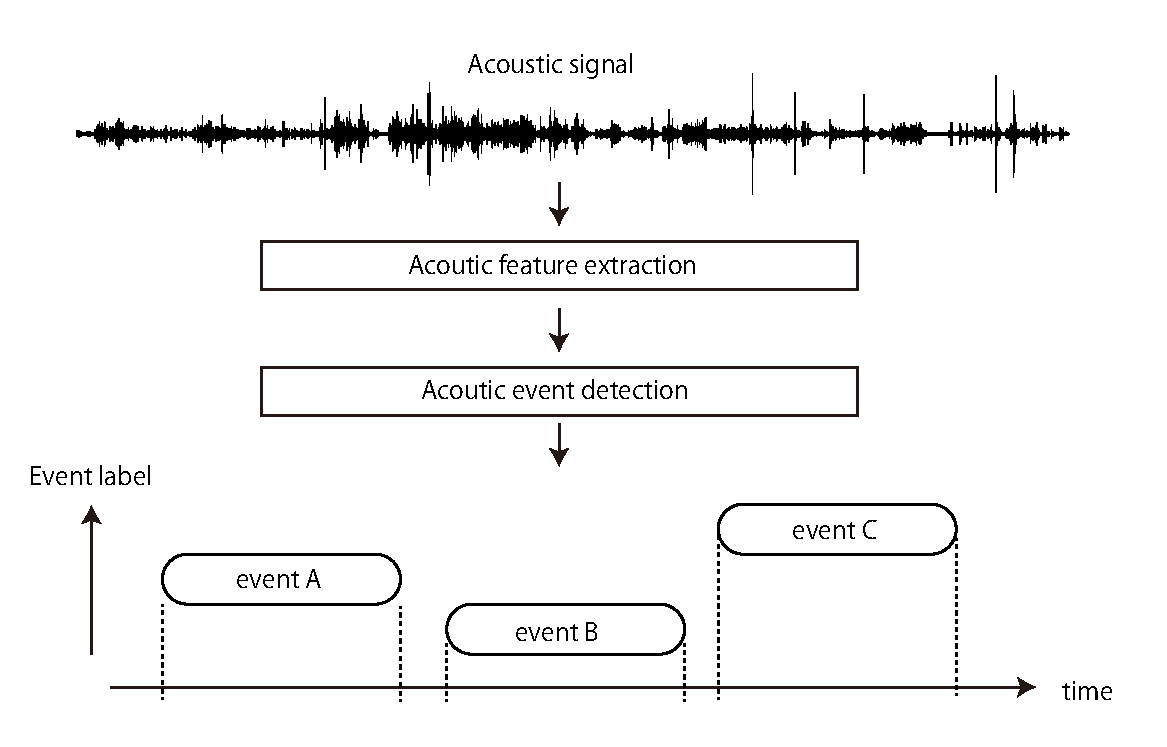
\includegraphics[width=8cm]{fig/aed_fig.pdf}
  \caption{Probrem of Acoustic event detection}
  \Description{}
  \label{aed}
\end{figure}

Cooking activities are fundamental to human life and supporting it with information processing technology will become more important in order to improve the quality of life\cite{Uriu2012}.

For speech information processing, support by a spoken dialogue system is considered, but in order to support cooking activities, it is necessary to recognize the state in a way that does not bother the cooker, and the question answering system is unsuitable. Therefore, it is necessary to recognize the states of cooking and use them for cooking activities understanding.

Studies using images or acceleration sensors for cooking activities recognition have been performed\cite{Torre2008}\cite{Shimada2013}\cite{Kuehne2014}.
However, studies using sounds (cooking sounds) generated at the time of cooking are performed only limitedly\cite{Kojima2016}, and research to tackle the recognition of the entire cooking process has not been conducted.

While image recognition is good at recognizing static objects such as food materials, cooking sounds are superior in recognition of cooking behavior such as "cutting" and "stir-frying", and it is suitable for this task.

Identification of cooking sound can be considered as a task of Acoustic Event Detection and Classification (AEDC) (Fig. \ref{aed}), but it is difficult to define the target to be recognized.
What can be thought of as a recognition unit is cooking behavior such as "cutting" or "stir-frying" as described in the recipe. However, in order to perform recognition in cooking behavior units, it is necessary to model cooking sounds labeled for each cooking behavior appropriately, and it is necessary to appropriately model cooking sounds labeled for each cooking behavior, A method that directly associates features is not suitable\cite{Maijala2018}.

In this research, assuming that the cooking sound when doing cooking behavior can be described by the overlapping pattern of the basis of plural sound events, by extracting the sound event feature amount by nonnegative matrix factorization and modeling it, cooking We examined whether it is possible to identify behavior.

\section{Related work}
% 関連研究
\subsection{Cooking Activities recognition}
% 調理行動認識関係の研究

% Egocentric videos を活用した調理行動認識の研究や調理中の画像データを活用した調理行動認識の研究が行われている.
Research on cooking behavior recognition using Egocentric videos and research on cooking behavior recognition using image data during cooking are being conducted. \cite{Urabe2018} \cite{Kuehne2014}.
% これらの研究では,調理中のデータとそれに対応するラベルデータを収集して実験・評価を行なっている.本論文でも同様に,調理中の音響データを収集し対応するラベルデータを手動で付与することでデータセットを構築し,実験・評価を行う.
In these researches, data during cooking and the corresponding label data are collected to conduct experiments and evaluations. Similarly in this paper, data sets are constructed by collecting acoustic data during cooking and manually assigning the corresponding label data, and experiments and evaluations are performed.

\subsection{Acoustic event detection}
% AEDの研究

% 音響イベント検出は鳥の鳴き声や銃声などの音響信号から知覚されるイベントを検出するテーマである.
Acoustic event detection is a theme that detects perceived events from acoustic signals such as bird calls and gunshots.
% 音声認識技術を応用して研究が行われてきたが,深層学習の技術発展により難しい問題にも取り組まれつつある.
Although research has been conducted by applying speech recognition technology, it is also addressing difficult problems by technological development of deep learning.
% 音響イベントの種類は多岐にわたるため,低質なデータセットを活用するための研究や小規模のデータセットを活用するための研究が課題である.
There are many types of acoustic events, so research for using low-quality data sets and research for using small-scale data sets are issues\cite{Imoto2018}.
% 調理中の環境音を含むデータセットは公開されていないため,本論文では新しくデータセットを構築し,実験・評価を行なった.
Since the data set including environmental sound during cooking is not released, in this paper, a new data set was constructed, and experiments and evaluations were performed.

\section{Proposed Method}
% 提案手法
\subsection{Feature extraction}
% 使用した特徴量について書く

% 本論文では2種類の特徴量を使用した.一つ目はMFCC,もう一つはNMFを用いたアクティベーション行列である.
In this paper, two feature quantities are used. The first is the Mel frequency cepstrum coefficient (MFCC), and the other is the activation matrix using Nonnegative Matrix Factorization (NMF).

% MFCCは音声認識分野で広く使用されている特徴量であるが,AEDの分野でも有効な特徴量として広く用いられている.
 MFCC is a feature that is widely used in the speech recognition field, but it is also widely used as an effective feature in the field of AED.

NMF is one of multivariate analysis methods aimed at decomposing nonnegative value data into additive constituents, and attracts attention in various fields in recent years There is technology to be \cite{Lee1999}.

NMF is applied to the analysis of acoustic signals. The input spectrogram $ V $ as a two-dimensional matrix of time-frequency and approximate it to the product of two matrices $ H, U $ ($ V \simeq HU $). One is called the basis matrix, and multiple characteristic spectral distributions that make up the original spectrogram are obtained. The other is called a weighting matrix, which indicates how much weight each basis vector is added at each time. Define the distance between $ V $ and $ HU $ and perform minimization to find $ H, U $.
Using the generalized Kullback-Leibler divergence as a distance function, find the stopping point by the auxiliary function method.

\subsection{Cooking state modeling}
% 環境音を用いた調理状態の学習
The spectral basis is expected to be the spectrum of sound events that occur frequently in cooking sounds. However, the recognition unit of cooking sound has a longer duration than these sound events. Therefore, we propose to model cooking behavior using the frequency of each sound event appearing in a long time interval corresponding to cooking behavior.

Divide the weight vector sequence $ {U_t} $ by the window length $ N $ to obtain the weight matrix sequence $ X_0, \ldots, X_L $.
The NMF basis histogram $ \bm{x} _i $ is obtained by summing the weight vectors for each weight matrix.

\begin{equation}
\label{hist}
	\bm{x}_i = \sum_{n=0}^{N-1} X_{i, n}
\end{equation}

, where $ X_ {i, n} $ is the nth row of the weight matrix $ X_i $.
The histogram $ \bm {x} _i $ of the cooking behavior $ A $ is modeled by the output probability distribution $ P (x | A) $.

\section{Experiment}
\subsection{Dataset}
The cooking sound data set was constructed. Different cooks cook in different environments to avoid over-learning by recording in a specific environment, and the recipe made for the sake of simplicity is the same as the recipe specified.
The specified food is "Yakisoba", which is Fried noodles. The recipe specified a simple one.
For recording, we used an iPhone 8 built-in microphone, and recorded using \SI{48}{kHz} sampling, and in the experiment we used downsampling to \SI{16}{kHz}. The recorded data is 6 times, about 130 minutes in total.
The labeling was done by the cook himself, and I asked them to fill in each section of the procedure described in the recipe.

\begin{figure}[t]
  \centering
  \begin{minipage}{0.48\hsize}
    \centering
    \includegraphics[width=3cm]{fig/ingredients.pdf}
    \subcaption{the ingredients}
  \end{minipage}
  \begin{minipage}{0.48\hsize}
    \centering
    \includegraphics[width=3cm]{fig/dish.pdf}
    \subcaption{the dish}
  \end{minipage}
  \caption{the ingredients and dish}
  \Description{}
  \label{yakisoba}
\end{figure}


\subsection{Frame by frame cooking state identification}
Four classification experiments were conducted to classify cooking noise into three classes: "Cut", "Fish", and "Other". A six-fold cross validation was performed using the six recorded data recorded. The probability density function for all experiments was Gaussian mixture model (GMM).
First, as a baseline, the cooking sound was converted to a feature sequence, and a discrimination experiment was performed assuming that each time frame always follows GMM (MFCC).
The feature is a 36-dimensional vector combining 12-dimensional MFCC with 1st-order and 2nd-order dynamic feature. Both frame length and frame shift are \SI{16}{ms}. Frames are grouped into segments so that the identification is performed for each segment.

Next, we tried soft clustering using GMM for all cooking sound data, and tried to generate a histogram using the class posterior probability for each frame (GMM). The mixture number of GMM was 20, and the histogram was set to be generated every second.

Third, we used the NMF basis histogram, which is the proposed method (NMF). The specified number of NMFs was 20, and the histogram was set to be generated every second.

Finally, in addition to the proposed method, we also examined a method for decomposing a spectrogram into two spectrograms before base decomposition with NMF (HPSS).

The decomposition method is intended to preserve the continuity in the time direction and the frequency direction respectively by median filter, and it is expected that the spectral basis will be learned appropriately by this.
The basis number of NMF was set to be 10 for each of two resolved spectrograms, and the histogram was generated every one second.
The mixing number of GMM was only 2 mixed with MFCC, and the other 3 methods were 32 mixed.

\begin{table}[t]
  \centering
  \caption{MFCC results}
  \label{result1}
  \scalebox{0.8}{
  \begin{tabular}{c|cccccc}
    \hline \hline
          & mix-1 & mix-2 & mix-4 & mix-8 & mix-16 & mix-32 \\ \hline
    val 1 & 61.84 & 63.70 & 65.79 & 72.60 & 70.35  & 74.50  \\
    val 2 & 48.55 & 68.33 & 60.70 & 65.99 & 64.69  & 62.11  \\
    val 3 & 59.67 & 60.30 & 61.56 & 63.23 & 54.67  & 56.10  \\
    val 4 & 63.52 & 69.48 & 75.28 & 54.64 & 55.19  & 55.01  \\
    val 5 & 77.15 & 78.60 & 79.70 & 79.62 & 81.07  & 80.80  \\
    val 6 & 65.72 & 69.61 & 80.12 & 71.90 & 74.64  & 77.15  \\ \hline
  average & 62.74 & 68.34 & 70.53 & 68.00 & 66.77  & 67.61  \\
    \hline \hline
  \end{tabular}
  }
\end{table}

\begin{table}[t]
  \centering
  \caption{NMF results}
  \label{result2}
  \scalebox{0.8}{
  \begin{tabular}{c|cccccc}
    \hline \hline
          & mix-1 & mix-2 & mix-4 & mix-8 & mix-16 & mix-32 \\ \hline
    val 1 & 57.98 & 65.12 & 67.29 & 66.49 & 66.68  & 70.21  \\
    val 2 & 50.41 & 65.92 & 66.20 & 66.71 & 67.84  & 72.39  \\
    val 3 & 56.49 & 58.04 & 51.86 & 48.26 & 52.40  & 54.49  \\
    val 4 & 49.91 & 61.18 & 62.85 & 47.88 & 32.88  & 32.98  \\
    val 5 & 56.15 & 72.58 & 74.98 & 71.07 & 75.32  & 70.80  \\
    val 6 & 51.29 & 57.46 & 52.44 & 51.83 & 60.00  & 55.86  \\ \hline
  average & 53.71 & 63.38 & 62.60 & 58.70 & 59.18  & 59.45  \\
    \hline \hline
  \end{tabular}
  }
\end{table}

The table \ref{result1} \ref{result2} shows the F value of each class and the whole for each method.

The MFCC method directly associates the acoustic features with the labels, and it is considered that the difference between various cooking environments was not successfully absorbed.
Moreover, the GMM method is characterized by the class posterior probability and is expected to be robust to differences in environment, but it has the lowest F value. This was the worst% result.
GMM learns that each time frame belongs to only one cluster, so unlike NMF where multiple bases are allowed to be included at the same time, cooking behavior could not be modeled well It is thought that there is no.
On the other hand, the proposed NMF method can model cooking behavior by the superposition pattern of sound events, and it is thought that good results have been obtained.
When HPSS is used in addition to the proposed method, it was expected that the basis could be learned more properly by separating the pulsing sound and the steady sound in advance. It was suggested that it did not fit the purpose of expressing the probability distribution of each action.



\subsection{Post processing}
% 制約を設けた結果について書く

% フレームごとの状態推定では状態が頻繁遷移してしまう点が問題である.これを回避する手法として HMM を用いて状態遷移に制約をつけることが一般に用いられる.
In frame-by-frame state estimation, the problem is that the state changes frequently. As a method to avoid this, it is generally used to constrain the state transition using HMM.
% 本論文では,単に状態遷移回数を既知として,状態遷移回数が正しくなるまで平滑化フィルタをかけるという手法を使用した.
In this paper, we use the method of simply making the number of state transitions known and applying a smoothing filter until the number of state transitions is correct.

\begin{figure}[t]
  \centering
  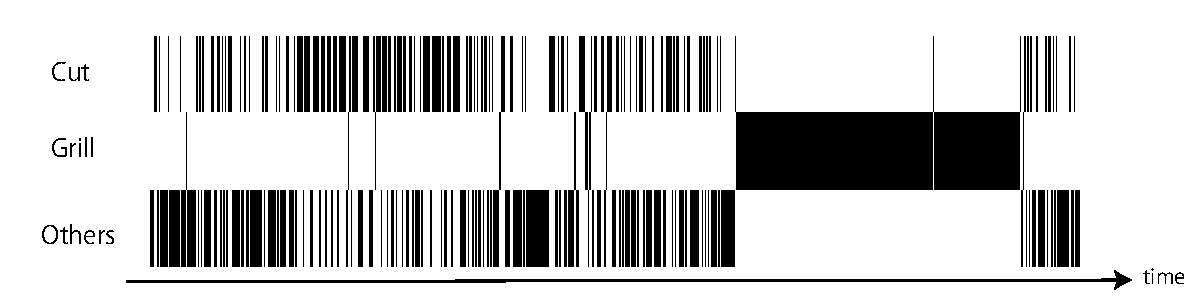
\includegraphics[width=8cm]{fig/N63_m4.pdf}
  \caption{}
  \Description{}
  \label{baseine_timeline_result}
\end{figure}

\begin{figure}[t]
  \centering
  
\includegraphics[width=8cm]{fig/N63_m4_smoothed.pdf}
  \caption{result}
  \Description{}
  \label{baseine_timeline_smoothed_result}
\end{figure}


\section{Conclusion}
In this research, we presented a method of utilizing acoustic signals for cooking activities recognition for cooking support systems, and examined cooking state identification using cooking sound with real environment data.

% 音声分野で広く用いられている MFCC と GMM を使用して 70パーセントを超える識別結果をえることができた.
% 調理状態を音イベントの出現分布でモデル化する手法は低い精度の結果となった.今後の更なる研究が求められる.
Using the MFCC and GMM widely used in the audio field, we could obtain over 70\% identification results.
The method of modeling the cooking state by the appearance distribution of the sound event resulted in low accuracy. Further research is required in the future.

% The acknowledgments section is defined using the "acks" environment (and NOT an unnumbered section). This ensures
% the proper identification of the section in the article metadata, and the consistent spelling of the heading.

% \begin{acks}
% This research was partially supported by the Ministry of Education, Science, Sports and Culture, Grant-in-Aid for Scientific Research (?), 20XX-20XX(JP18K11369).
% \end{acks}

%
% The next two lines define the bibliography style to be used, and the bibliography file.
\bibliographystyle{ACM-Reference-Format}
\bibliography{reference}

% If your work has an appendix, this is the place to put it.
% \appendix

\end{document}
